% \documentclass[../main.tex]{subfiles}

% \begin{document}


\section{Evaluation} \label{section:evaluation}
We first describe some important training parameters, then describe the benchmark and the dataset for training, and finally we analyse the the experimental results. 


\subsection{Model parameters}
The implementation is based on the framework tf2\_gnn \footnote{\url{https://github.com/microsoft/tf2-gnn}}. We set the all middle layer sizes in the framework to 64, the number of message passing steps to 8 (i.e., apply Eq.~\ref{eq:hyperedge-GNN-definition} 8 times), the maximum training epoch to 500, and the patient to 100. For the rest of parameters, we use the default settings in the framework tf2\_gnn. 


\subsection{benchmarks and dataset}
The dataset we used for training and evaluation is specified in Table~\ref{benchmark-table}. The models are trained by the labeled dataset, and it is divided to train, valid, and test set by 60\%, 20\%, and 20\%. The dataset is available in a Github repository\footnote{\url{https://github.com/ChenchengLiang/Learning-abstract-predicate-dataset}}

\import{tables/}{t1}



\subsection{Experimental results}
The measurements are number of solved problems and the solving time for solvable problems.

\import{tables/}{t2}


\begin{figure}[t]
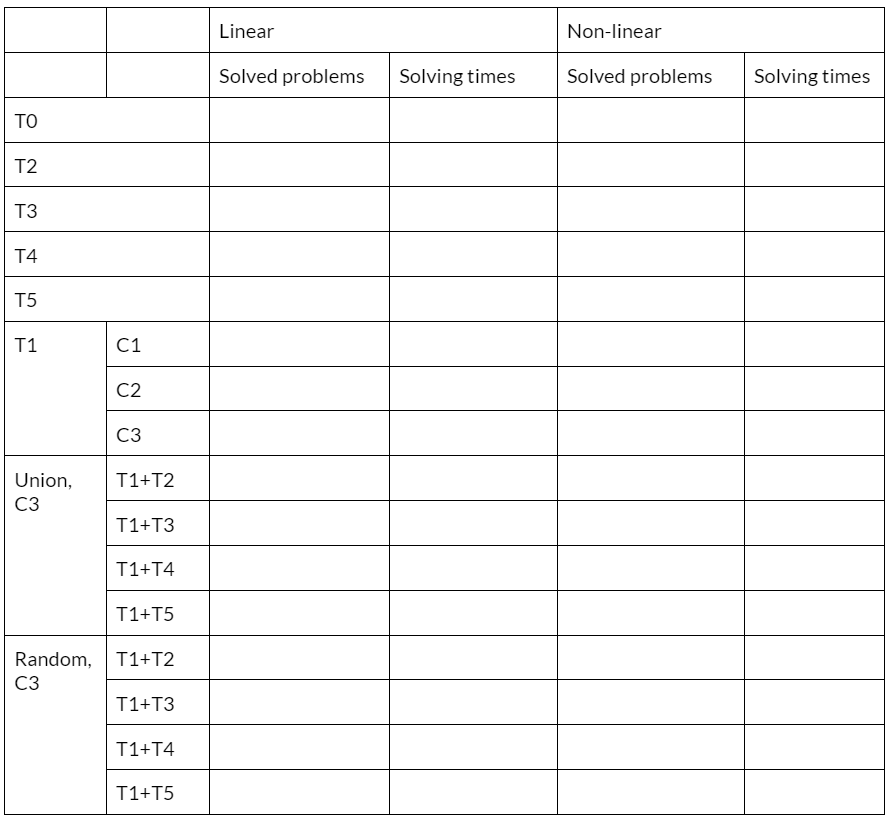
\includegraphics[width=\textwidth]{figures/Snipaste_2022-09-28_11-54-25.png}
\caption{T0 means no template is used, T1 is GNN-selected templates, T2-5 are templates from~\cite{Leroux2016}, and C1-3 are ways to assign cost value to GNN-selected templates. Union means combine the generated new predicates when use the two template sets. Random means use either the two template sets to generate the templates. } \label{fig:results}
\end{figure}




%limitation
 




% \end{document}


